\documentclass[11pt, letterpaper]{article}
\usepackage[backend=bibtex]{biblatex}
\bibliography{bib}
\usepackage[utf8]{inputenc}
\usepackage{amsmath}
\usepackage{amsfonts}
\usepackage{amssymb}
\usepackage{fullpage}
\usepackage{lmodern}
\usepackage{graphicx}
\usepackage{gensymb}
\usepackage{parskip}
\author{Revan~Sopher}
\title{Detecting Planes in Real-Time for Camera Display Communications\\
{\large Independent Study Report}}
\begin{document}
\maketitle

\begin{abstract}
TODO
\end{abstract}

\section{Introduction}

\subsection{Visual MIMO}
The aim of the Visual MIMO project thus far has been to embed messages within images by varying the intensity of patches of the image, and to reliably extract these messages from pictures of the image displayed on a screen.

The existing software system is capable of detecting the computer monitor, in order to to consider only the displayed image, but encounters difficulties with the variance in photometry dependent on camera and display type, and the spatial positioning of the two.
This is addressed via radiometric calibration: nearly invisible patches are created on the corners of the image using histogram equalization, creating calibration data.

TODO: expand

\subsection{Mobile Challenges}
Although the Visual MIMO project is intended to make use of the ubiquity of handheld cameras, previous work has been reliant on a precise, static configuration of high quality SLR camera and a desktop computer.
The purpose of this independent study will be to facilitate the implementation of this algorithm to run on a mobile device, such as a smartphone or Google Glass.
This will require special considerations and optimizations to compensate for the significantly weaker processor and average cameras: the processing limitations can be mitigated by lower level programming and memory management using the Android Native Development Kit, but the lower quality image and light sensors may need experimentation.

The primary focus of this study is in addressing the issues that arise from the spatial differences between the camera and the screen: although radiometric calibration can mitigate such differences, the resulting calibration is only valid for the current positions, resulting in a fragile setup unsuitable for casual demonstrations.

The goal is to increase the accuracy of imperfect positioning, without requiring explicit calibration.

\section{Image Tracking with Vuforia}
The Android application is built around the Qualcomm Vuforia SDK \cite{vuforia}, a library meant for facilitating the construction of Augmented Reality applications.
Vuforia is used for its image tracking capabilities: known "targets" are trained ahead of time, and are quickly and reliably detected in realtime.

Upon detection,	Vuforia provides the pose matrix. Combined with the known size of the target image, we can calculate the position of the image corners.

\section{Native Image Processing}
\subsection{Image Format}
The camera image is encoded in RGB888, meaning a one dimensional array of tuples of red, grean, blue values from 0 to 255.
This format was selected over alternatives for its large information quantity.

\subsection{Skew Correction}
The usage of a mobile device for image capture necessarily forecloses angular calibration.
As such, the image captured is usually not head on (Figure~\ref{fig:skew}).
In this step, we use a projective transformation to correct for skew.

First we obtain the $3 \times 3$ transformation matrix, such that:

$$
\begin{pmatrix}
t_i x_i^*\\
t_i y_i^*\\
t_i
\end{pmatrix}\\
= \text{transformation\_matrix} \cdot
\begin{pmatrix}
t_i x_i\\
t_i y_i\\
1
\end{pmatrix}
$$
That is, we map each corner to the proper rectangular positions.

Having calculated the corner positions previously and knowing the shape of the original image, this is easily accomplished with OpenCV\cite{opencv_getperspectivetransform}.

Next, we apply the transformation by multiplying the found matrix with each point in the image.
This is again straightforward with OpenCV \cite{opencv_warpperspective}, yielding Figure~\ref{fig:skew2}.

\begin{figure}[hbtp]
\centering
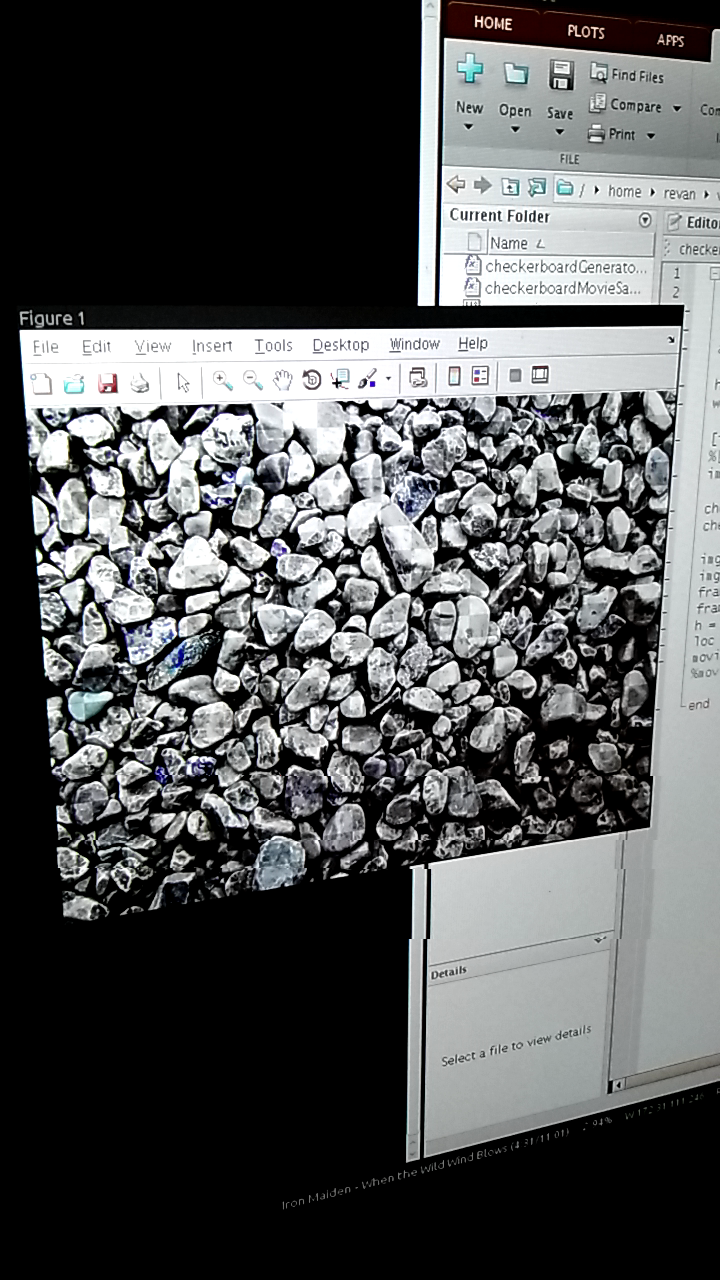
\includegraphics[scale=0.10]{img/skew.png}
\caption{An image viewed at an oblique angle.}
\label{fig:skew}
\end{figure}

\begin{figure}[hbtp]
\centering
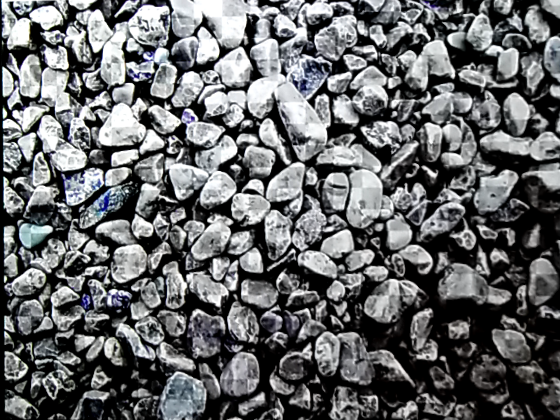
\includegraphics[scale=0.2]{img/skew2.png}
\caption{The image, skew-corrected by projective transformation.}
\label{fig:skew2}
\end{figure}

\subsection{Histogram Equalization}
In the histogram equalization step, we improve the image contrast and transfer faithfulness by ``stretching'' the pixel intensity histogram to resemble a normal distribution (Figure~\ref{fig:histogram}).

Optimally we apply the same transformation to both images, however this is not especially straightforward using OpenCV so we rely on the two images having similar transforms and run the histogram equalization function twice.

The source image is histogram equalized before encoding and in decoding, which helps? TODO
\begin{figure}[hbtp]
\centering
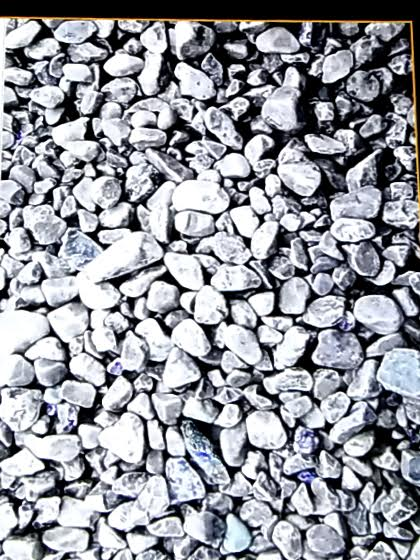
\includegraphics[scale=0.2]{img/histeq1.jpg}
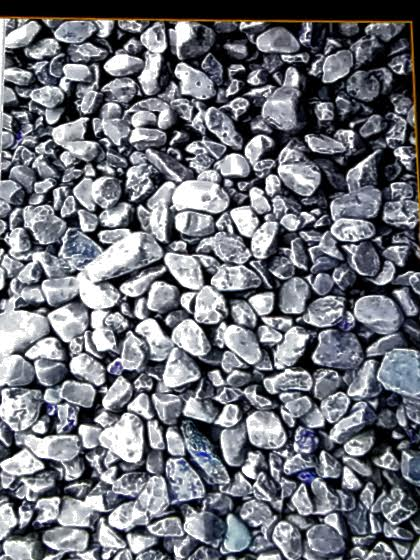
\includegraphics[scale=0.2]{img/histeq2.jpg}
\caption{An example of histogram equalization of an image: original on the left.}
\label{fig:histogram}
\end{figure}

\subsection{Subtraction}
With both targets skew-adjusted and normalized, we subtract one image from the other:

$$\text{dst}[I] = \text{saturate}(\text{src1}[I] - \text{src2}[I])$$ where $I$ is the image matrix\cite{opencv_subtraction}.

As the non-message part of the images should match up, this should leave only the message (Figure~\ref{fig:subtract}).

\begin{figure}[hbtp]
\centering
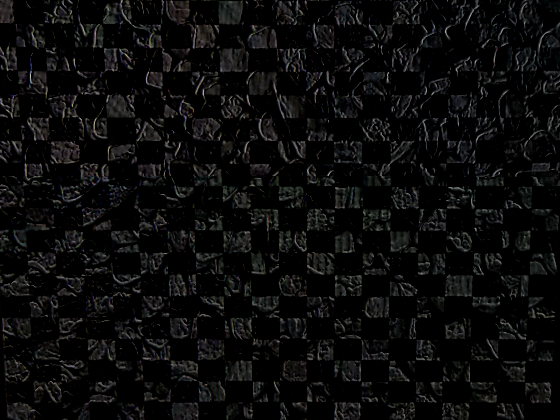
\includegraphics[scale=0.2]{img/subtract.png}
\caption{An example of subtraction.}
\label{fig:subtract}
\end{figure}

\subsection{Information Extraction}
Having isolated the encoded pattern, we must then decode the information inside.

We divide the difference image into a grid, and compare the average intensity of each quadrant against the average intensity of the entire image.
Assuming a even distribution of 1's and 0's, the average intensity of the entire image will be approximately halfway between the ``on'' and ``off'' intensities.

\section{Accuracy Benchmark}
Accuracy is evaluated by encoding a known random binary string, and testing the errors in transmission.

\subsection{Results}
TODO

\section{Synchronization}
Earlier iterations of the system had no synchronization measures in place, so the two frames chosen for subtraction were often not properly matched.
Combination such as both frames displaying the message added, or both subtracted, lead to unusable resulting images.
The system also breaks when encountering frames that are between clean updates on the screen.

\subsection{Sliding Window}
This synchronization method involved taking four frames rather than just two, and selecting the best two frames to perform the subtraction and extraction on.
For each frame, we calculate the average intensity, and select the combination of two frames which maximizes the absolute value of the difference of their intensities.
We estimate that the refresh speed of the camera is ~20 FPS, so we fix the refresh speed of the encoded message at 10 FPS, the Nyquist frequency for this camera.

The reasoning for this method is based on the idea that the transitions between frames on the display are non-instantaneous, causing inaccuracies in decoding.
By sampling at twice the rate of the display, we can be reasonably sure that we will capture at least one clean picture of both states of the frame. (Figure~\ref{fig:slidingwindow}).

\begin{figure}[slidingwindow]
  \centering
  TODO
  \caption{Illustration of the Sliding Window}
  \label{fig:slidingwindow}
\end{figure}


\subsection{Multi-frame Messages}
The implementation described thus far only allows for as much information as can be encoded into a single image.
In order to scale this prototype arbitrarily, we must be able to encode and decode a series of messages sequentially.

To this end, the last few blocks of the message are reserved for an index giving the position of the message relative to the other messages.
TODO

\section{Google Glass}
Porting to Google Glass poses several problems. Primarily, the processing capabilities are limited: not only is the processor weaker, but the heat generated by performing heavy computations locally causes the device to overheat.
Therefore, the ``proper'' approach to such an application on Google Glass would consist of offloading all processing to a server, however this means such an implementation is less technically interesting.

\printbibliography
\end{document}
